\chapter{Descrição das Atividades Realizadas}
\label{cap:atividades}

Este projeto tem como objetivo remover a funcionalidade de onboarding de clientes no ERP
do contratante do projeto, buscando simplificar a arquitetura do sistema. 
Atualmente, essa funcionalidade inclui integrações com birôs externos para 
verificar se o score de inadimplência do cliente está dentro do intervalo tolerado, 
além de uma integração com uma IDTech para validar a identificação do cliente 
durante o processo de onboarding, que envolve a captura de selfie e dos documentos 
de identificação, bem como a sincronização da base de dados  de clientes com a 
processadora do cartão.

Para atender a essas necessidades e simplificar a arquitetura do sistema, 
foi elaborada uma solução baseada em microsserviços. 
A \autoref{arquitetura-projeto} ilustra a arquitetura proposta, 
onde cada microsserviço é responsável por uma parte do processo de onboarding, 
garantindo maior escalabilidade e facilidade de manutenção. Nas subseções seguintes, 
cada um desses microsserviços será detalhado, explicando sua 
função e como interagem entre si.


\begin{figure} [!h]
    \centering
    \caption{Arquitetura do projeto}
    \includegraphics[width=1\textwidth]{arquivos/imagens/Arquitetura-relatório-estágio.png}
    \label{arquitetura-projeto}
    \legend{Fonte: próprio autor }
\end{figure}

\section{Broker}

Microsserviço cuja finalidade é atuar como um broker, que é um  
componente centralizado que gerencia a comunicação entre diferentes partes do sistema \cite{distributed:systems:book}. 
Seguindo esse conceito, o broker funcionará como intermediador na comunicação entre os 
serviços internos e a processadora do cartão, que é um serviço externo. 
Esse microsserviço é essencial para o ecossistema, pois evita a duplicação de 
configurações de integração nos microsserviços que dependem dos dados da processadora 
de cartão.

\section{Onboarding}

O onboarding é um microsserviço que foi implementado utilizando SpringBootWeb aderindo ao padrão MVC, disponibilizando 
uma API que visa informar o fluxo de crédito que o cliente deve seguir quando solicita um cartão, 
que são respectivamente: 
\begin{enumerate}
    \item \textbf{Nova proposta}: Quando o cliente não possui inadimplências, carnê ou cheque e não possui o cartão informado. 					
    \item \textbf{Reanálise de crédito}: Quando o cliente possui o cartão, porém está bloqueado por inatividade de compras por 12 meses.
    \item \textbf{Reprovado}: caso possua inadimplências, carnê ou cheque, ou possua o cartão ativo, ou possua o cartão bloqueado, porém o tipo de bloqueio diferente de inativação. 
\end{enumerate}

A \autoref{fluxo-onboarding} ilustra o diagrama de fluxo do microsserviço de onboarding de clientes, detalhando as 
quatro etapas principais desse processo: captação de proposta, verificação de 
inadimplências, consulta à processadora de cartão e tomada de decisão final. 
A seguir, cada uma dessas etapas será descrita em detalhes, evidenciando a lógica e as interações entre os componentes do sistema.

Após o solicitante da proposta informar o \textbf{cpf} e o \textbf{cartão desejado} no 
\textbf{sistema de captação de proposta}, essas informações são
encaminhadas ao microsserviço de \textbf{onboarding}. Este, por sua vez, 
consulta o banco de dados do contrante do projeto para verificar a existência de 
pendências financeiras a partir do cpf. 

Caso sejam identificadas inadimplências, o \textbf{sistema de captação de proposta} é notificado para reprovar a proposta.
Se o cliente estiver em dia com suas obrigações, o \textbf{onboarding} realiza uma consulta ao broker utilizando o \textbf{cpf} do cliente. 

O \textbf{broker}, atuando como intermediário, encaminha essa solicitação à \textbf{processadora de cartão},
que retorna as informações cadastrais do cliente. Com os dados obtidos, o \textbf{onboarding} verifica se o cliente já possui o cartão solicitado.

Caso o cliente ainda não possua o cartão, o \textbf{sistema de captação de proposta} é notificado para seguir o 
fluxo de nova proposta. No entanto, se o cliente já possui o cartão, 
o \textbf{onboarding} verifica o status da conta. Se a conta estiver inativa o 
\textbf{sistema de captação de proposta} é notificado para seguir o fluxo de reanálise de crédito. 
Caso contrário, \textbf{sistema de captação de proposta} é notificado para reprovar a proposta.

\begin{figure}
    \centering
    \caption{fluxo do onboarding}
    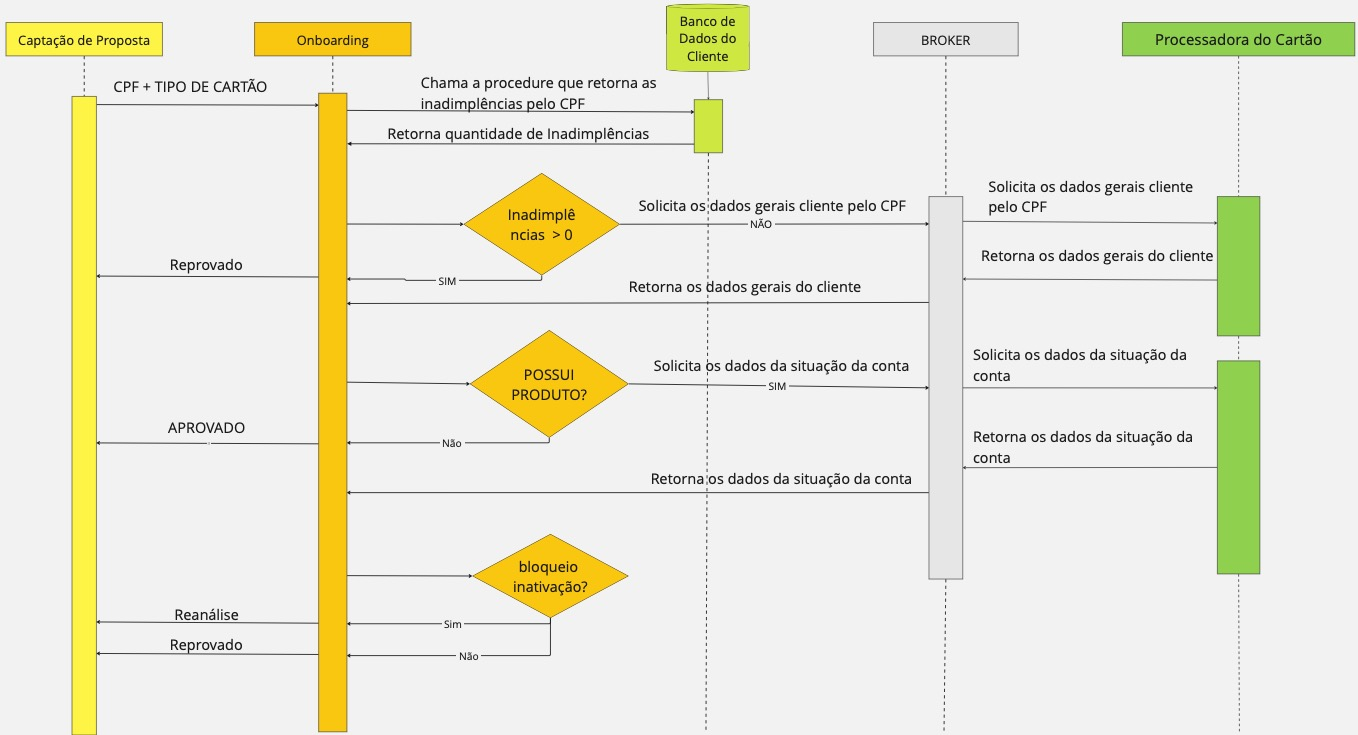
\includegraphics[width=1\textwidth]{arquivos/imagens/onboarding-fluxo.jpg}
    \label{fluxo-onboarding}
    \legend{Fonte: próprio autor }
\end{figure}

O microsserviço de onboarding desempenha um papel crucial na gestão de riscos e na otimização da carteira de clientes. 
Ao impedir a concessão de crédito a indivíduos com histórico de inadimplência, a empresa minimiza o risco de 
inadimplências futuras, protegendo seu patrimônio. Além disso, o sistema incentiva a aquisição do cartão de crédito 
pela loja, desestimulando o uso de outras formas de pagamento, como o carnê, o que contribui para o aumento da 
rentabilidade e da fidelização dos clientes.

\section{Cadastro/Atualização de cliente}

O cadastro/atualização de cliente é um microsserviço, que foi implementado utilizando framework SpringBootWeb e 
seguindo a arquitetura MVC, disponibilizando uma API responsável por processar as propostas aprovadas e encaminhar 
os dados do cliente para um processo de cadastro de nova conta ou atualização dos dados na base de dados do 
contrante do projeto.

A \autoref{fluxo-Cadastro-Atualizacao} ilustra o diagrama de fluxo do microsserviço de cadastro/atualização de cliente, 
detalhando as três etapas principais desse processo: recepção de propostas aprovadas, validação e 
atualização dos dados do cliente e, por fim, o armazenamento das informações no banco de dados. 
A seguir, cada uma dessas etapas será descrita em detalhes, evidenciando a lógica e as interações entre os 
componentes do sistema. 

\begin{figure} [!h]
    \centering
    \caption{fluxo do cadastro/atualização de cliente}
    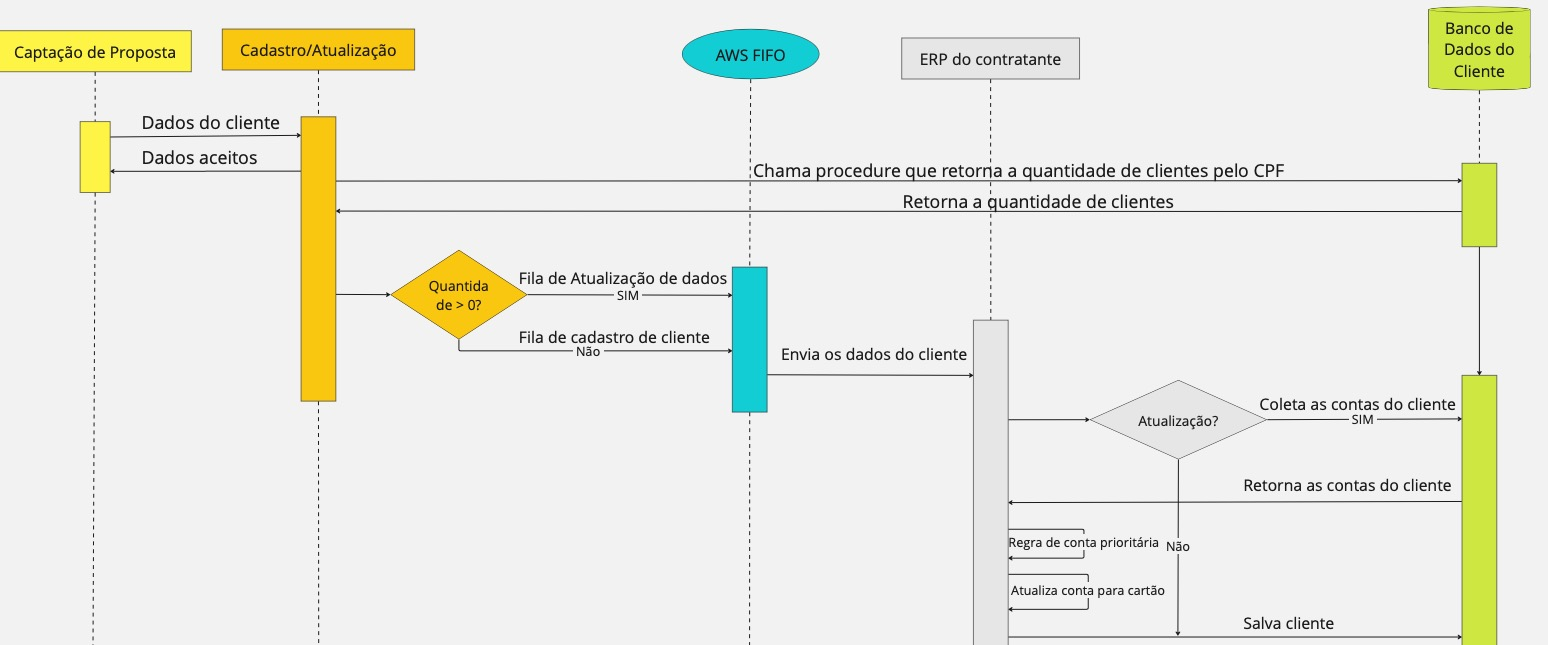
\includegraphics[width=1\textwidth]{arquivos/imagens/Cadastro-Atualizacao-fluxo.jpg}
    \label{fluxo-Cadastro-Atualizacao}
    \legend{Fonte: próprio autor }
\end{figure}

Após a avaliação do perfil de crédito pelo microsserviço de onboarding, 
o cliente é direcionado para um dos seguintes fluxos de proposta: 
nova proposta ou reanálise de crédito. 
Para a aprovação da proposta, é necessário passar por duas etapas:
\begin{enumerate}
    \item \textbf{Verificação de crédito}: É realizada uma consulta aos birôs de 
    crédito para avaliar o score de inadimplência do cliente. 
    Caso o score esteja dentro do limite permitido, o cliente avança 
    para a próxima etapa.
    \item \textbf{Atualização cadastral e validação biométrica}: O cliente 
    atualiza seus dados cadastrais e realiza a captura de uma selfie para fins 
    de validação biométrica caso estiver no fluxo de nova proposta.
    Após essa etapa as informações preenchidas são 
    submetidas para o sistema de reconhecimento facial e documental (IDTech). 
    Caso sistema identifique alguma inconsistência, a proposta é reprovada.
\end{enumerate}

Após a aprovação, os dados da proposta são enviados ao microsserviço de 
cadastro/atualização. O microsserviço consulta a base de dados para verificar a 
existência de um cadastro associado ao cliente. Se o cadastro for encontrado, 
os dados da proposta são encaminhadas para a fila de atualização. 
Caso contrário, os dados da proposta é enviada para a fila de cadastro.

O sistema de ERP, ao receber a mensagem da fila, 
processa a solicitação, realizando o cadastro completo do
cliente ou a atualização dos dados existentes, vinculando à conta ao tipo de 
cadastro fatura. Ao atualizar os dados de um cliente com múltiplas contas, 
o sistema escolhe a conta com o tipo de cadastro que deve ser priorizada para 
o processo de atualização descartando as outras na seguinte ordem: 
fatura, carnê e por último cheque ou cartão de crédito/vista(não pertence ao contrante do projeto).

O microsserviço de cadastro/atualização desempenha um papel crucial na manutenção 
da integridade dos dados do cliente, evitando a duplicidade de contas e indicando 
ao ERP qual a ação a ser tomada: cadastro ou atualização. Essa integração com o ERP permite a migração  de contas de outros tipos de 
pagamento (carnê, cheque, cartão de crédito/vista) para o cartão próprio do 
contratante do projeto. 

Essa migração oferece benefícios ao contratante 
do projeto, como: maior comodidade na gestão de pagamentos, disponibilizar 
benefícios exclusivos ao uso do cartão, ofertar programas de pontuação e 
condições especiais, fortalecendo assim o vínculo com a empresa e aumentando a 
probabilidade de novas aquisições. Além de \textbf{transferir} a responsabilidade da gestão 
dos dados do contrante do projeto para a processadora do cartão.

\section{Rotina de inativação de cliente}

A rotina de inativação é um microsserviço que foi implementado utilizando o 
framework SpringBootWeb aderindo ao padrão MVC, que tem como objetivo bloquear 
clientes que estão a mais de 12 meses sem comprar no cartão de crédito.

A \autoref{fluxo-rotina-inativacao} ilustra o diagrama de fluxo do microsserviço 
de rotina de inativação, detalhando as três etapas principais desse processo: 
download de arquivo com clientes que devem ser bloqueado, verificação dos status 
da conta na processadora do cartão e, por fim, o bloqueio do cliente. A seguir, 
cada uma dessas etapas será descrita em detalhes, evidenciando a lógica e as 
interações entre os componentes do sistema. 

\begin{figure} [!h]
    \centering
    \caption{fluxo da rotina de inativação}
    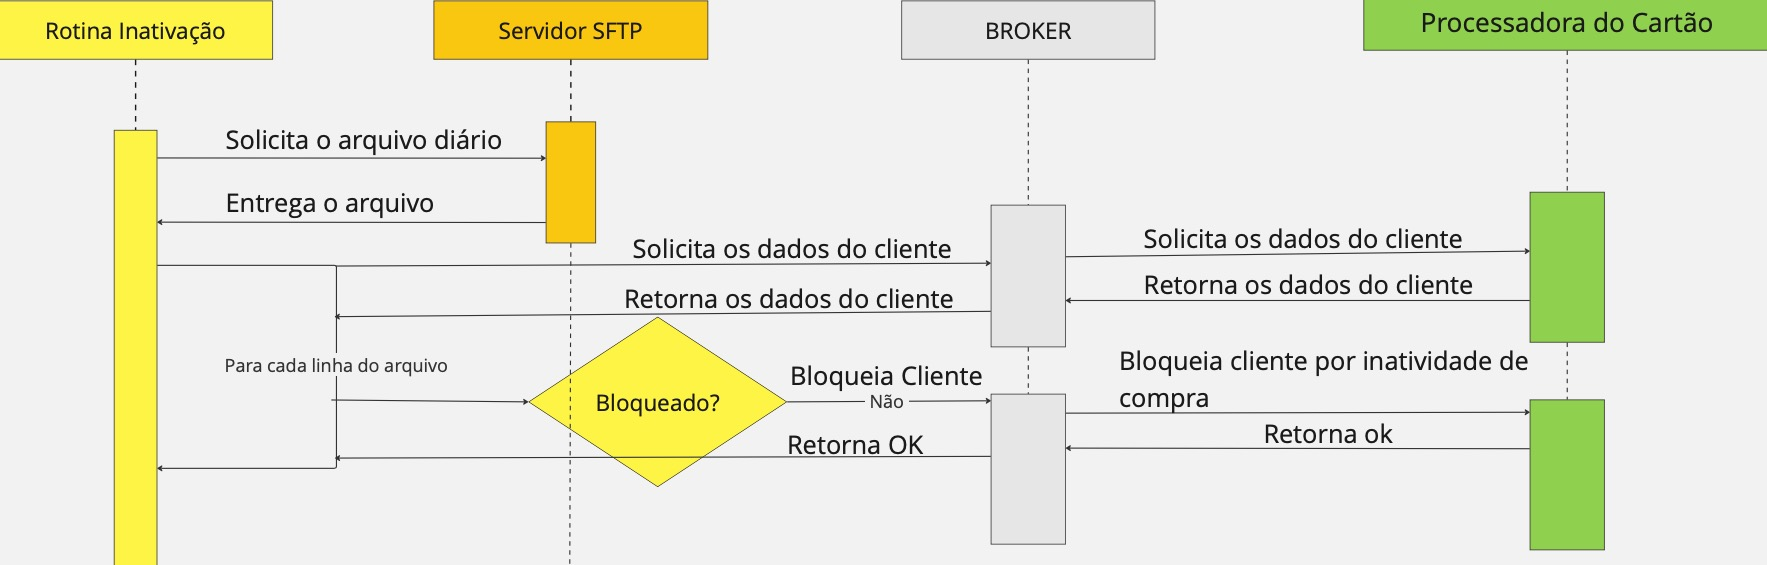
\includegraphics[width=1\textwidth]{arquivos/imagens/fluxo-rotina-inativacao.jpg}
    \label{fluxo-rotina-inativacao}
    \legend{Fonte: próprio autor }
\end{figure}

O microsserviço de rotina de inativação disponibiliza um job diário agendado às 
00:00 a fim de baixar um arquivo CSV com uma lista de clientes que devem ser 
bloqueados com o tipo de bloqueio de inativação há mais de 12 meses sem compras no 
servidor SFTP. 

Para cada cliente na lista, o job consulta o broker para obter as informações sobre 
a conta do cliente que por sua vez encaminha para a processadora do cartão. Caso a 
conta esteja ativa, o job envia uma solicitação ao broker para bloquear a conta do cliente, 
que por sua vez encaminha para a processadora do cartão.

O microsserviço de rotina de inativação desempenha um papel importante para a 
manutenção  do processo de reanálise de crédito no sistema de captação de proposta, 
pois esse processo só ocorre em clientes com bloqueio de inativação de 12 meses. 
Permitindo também identificar clientes inativos, a fim de analisar o seu comportamento,
possibilitando a criação de programas de incentivo personalizados para estimular 
novas compras.
